\chapter{Discussion}
In this chapter the developed solutions and the results are discussed from different aspects. Problems, which occured during the bachlor thesis, are presented as well.

\section{Cell as a sphere}
To draw a sphere cell is one way to get the desired spherish shape of the cell. Sadly, to keep the shape of the cell during the growth process does not work. Because for a given volume and a given surface there are all kinds of shapes \ac{CC3D} does not know which shape the cell should have. It it suprising that every time during the growth process the cells get a shape similiar to a cube. It might be a result of the square lattice, which is used in the simulation. Another interesting fact that is that smaller sphere cells get a form of a cube faster during the growth process than sphere cells with a larger radius. This might be a result of the larger radius. Figure \ref{img:GrowthSphereCellRadius5} and \ref{img:GrowthSphereCellRadius9} at page \pageref{img:GrowthSphereCellRadius5} and \pageref{img:GrowthSphereCellRadius9} display such an fact. It is observable that the cell with a radius of 5, at illustration \ref{img:GrowthSphereCellRadius5}, has a form of a cube after 50 \ac{MCS} whereas the larger sphere cell get a form like a cube after 250 \ac{MCS}. A sphere cell with a smaller radius has less details and therefore it is easier that this one is formed into a cube than a sphere cell with a larger radius. \newline
There are several research papers, which use \ac{CC3D} for their simulation, sadly it is never explained how the desired cell form is achieved neither which lattice type is used. Some of the literature is linked at the hompage of \ac{CC3D} \cite{CC3D.org}. So far, it is not possible to know if there is an mistake in the simulation or if the cells get shape similiar to a cube due to the square lattice. \newline
Because \ac{CC3D} only determines the shape of the cells, there are other techniques to reach the shape of a sphere for the cells. It is possible that a cell reaches a desired volume and surface, by only setting the terms for the volume and surface of the effective energy. The desired values can be reached faster if a high multiplier, $\lambda_{vol}$ and $\lambda_{sur}$, is set. This has the disadvantage that a volume or an surface constraint might weigh more than the term of the adhesion in the effective energy. If the specific multiplier has a small value, it might be possible that it takes a long time until the desired shape is reached. In addition to the volume and surface constraint comes the adhesion. The new adhesion matrix is discussed in the next section.

\section{Adhesion}
Adhesion influences the shape of two or more cells, as it describes how strong the cells stick to each other. If the adhesion is set too high the cells infiltrate each other but if it is too low the cells may not stick to each other as they change their shape. An example therefore is displayed at figure \ref{img:InfiltratingCells} at page \pageref{img:InfiltratingCells}. During the simulations with the old adhesion matrix it was observable that some cells of different cell types want to infiltrate each other. This is a result of to high adhesion. With the new adhesion matrix it still appeared that sometimes cells want to infiltrate each other. With the new adhesion matrix, displayed in table \ref{tbl:NewAdhesion} at page \pageref{tbl:NewAdhesion}, the adhesion energy between the cells is already loosened up. Because the adhesion was observed with two cells in a simulation field it might that this observation is not precise enough to be used in the simulation. This would be a reason that in a simulation the cell is sourrunded by other cells and therefore the results of the observation might not completely apply during a simulation. To find the perfect suiting adhesion values observations during simulations should be made. The problem is that this technique is too time comsuming as it would be useful. Maybe it is already enough to reduce the adhesion between the cell types, in which the cells wanted to infiltrate each other, but maybe it is also required that additional observations of the different adhesion values has to be made.

\section{Voxel Density}\label{sec:vD}
In the simulations the voxel density should be set to 1. In this case, in \ac{CC3D} one \SI{1}{\micro\metre} is presented by one voxel. If the voxel density is higher than one voxel represents less \SI{}{\micro\metre}. Because the simulations requires a lot of more time if the voxel density is high and the deviation between the volume and surface values of a sphere cell and a real sphere is larger, it should be tried to keep the voxel density as small as possible but also not to small. If the voxel density is too small than less details can be displayed and it is much more likely that the cells do not look like spheres. Why the deviation of the volume of a cell and a real sphere grows so much more for a higher voxel density, as it is displayed in figure \ref{img:DeviationSphereCellRealSphere-vD2}, is a puzzle. \newline
On one hand the deviation of the volume and the surface grows with the radius, with more voxels. Since with a higher voxel density there are also more voxels to display it might is a result that \ac{CC3D} uses more voxels to display the cell. On the other hand, with a voxel density of 2, the volume and surface values of the drawn cell are that high that for the surface of a real sphere a factor of six would give an approximation to the surface of the drawn cell. \newline
The surface of the cell is one factor, but as it is displayed in table \ref{tbl:CellConstraints} at page \pageref{tbl:CellConstraints} the correct volume is more important than the surface. In figure \ref{img:DeviationSphereCellRealSphere-vD2} the volume of a real sphere and of a drawn sphere cell in \ac{CC3D} is too far apart as this voxel density is useful for a simulation. It is interesting to observe that the volume of a sphere cell increases this fast, whereas the surface of a sphere grows in an almost linear way for an increasing radius. Since in \ac{CC3D} in a 3D simulation the volume refers to a physical volume and the surface refers to a physical surface it might be that one voxel still represent \SI{1}{\micro\metre}, even it should be only \SI{0.5}{\micro\metre}. This might explain the results, as they are similiar to the results of $2 \cdot r$ if the voxel densitiy is 1. \newline
As a voxel density of 2 is not useful for the simulation, the same case happens with a voxel density of 0.8. As it is displayed in figure \ref{img:DeviationSphereCellRealSphere-vD0,8} at page \pageref{img:DeviationSphereCellRealSphere-vD0,8} the surface of a real sphere and a sphere cell do match but the volume of the sphere cell does not grow fast enough. Because the volume of the sphere cell does not grow fast enough it deviates more with a growing radius to the volume of a real sphere. \newline
Image \ref{img:DeviationSphereCellRealSphere-vD1} at page \pageref{img:DeviationSphereCellRealSphere-vD1} display how well the volume of a sphere and a sphere cell in \SI{}{\micro\metre} fit for a voxel density of 1. For this voxel density the volume of the sphere and the sphere cell are so close to each other that there is no visible deviation in the image. In this image an further reaching radius was chosen to demonstrate this fact.

Because there is almost no difference between the volume of a sphere and a sphere cell the voxel density of 1 should be used in the simulation. Another advantage of this voxel density is that no convertion errors between the voxel unit and the physical unit in \SI{}{\micro\metre} can occur. \newline
Why the volume and surface values of a sphere and a sphere cell deviate different for the different voxel densities is a mystery. The values of a sphere cell for all three voxel densities are taken only of the by \ac{CC3D} drawn cell. Because the values are calculated by \ac{CC3D} it is possible that it is their mistake but it is also possible that the different deviations are normal and they were not discovered or explained in the literature yet.
\begin{figure}[ht]
	\center
	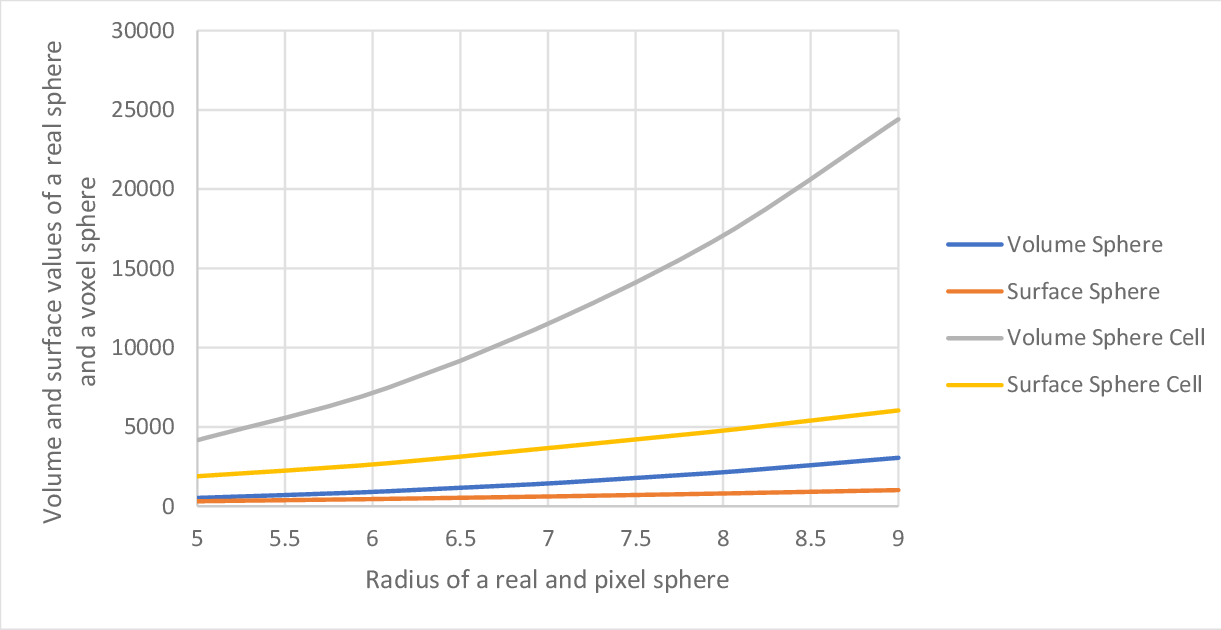
\includegraphics[scale=0.3]{figures/DeviationSphereToPixelSphere-vD2.png}
	\caption[Volume and surface in \SI{}{\micro\metre} between a sphere and a sphere cell for a voxel density of 2]{Volume and surface in \SI{}{\micro\metre} between a sphere and a sphere cell for a voxel density of 2. The lines 'Volume Sphere' and 'Surface Sphere' are displaying the volume and the surface of a sphere. The lines 'Volume Sphere Cell' and 'Surface Sphere Cell' display the volume and the surface of a sphere cell.}
	\label{img:DeviationSphereCellRealSphere-vD2}
\end{figure}

\begin{figure}[ht]
	\center
	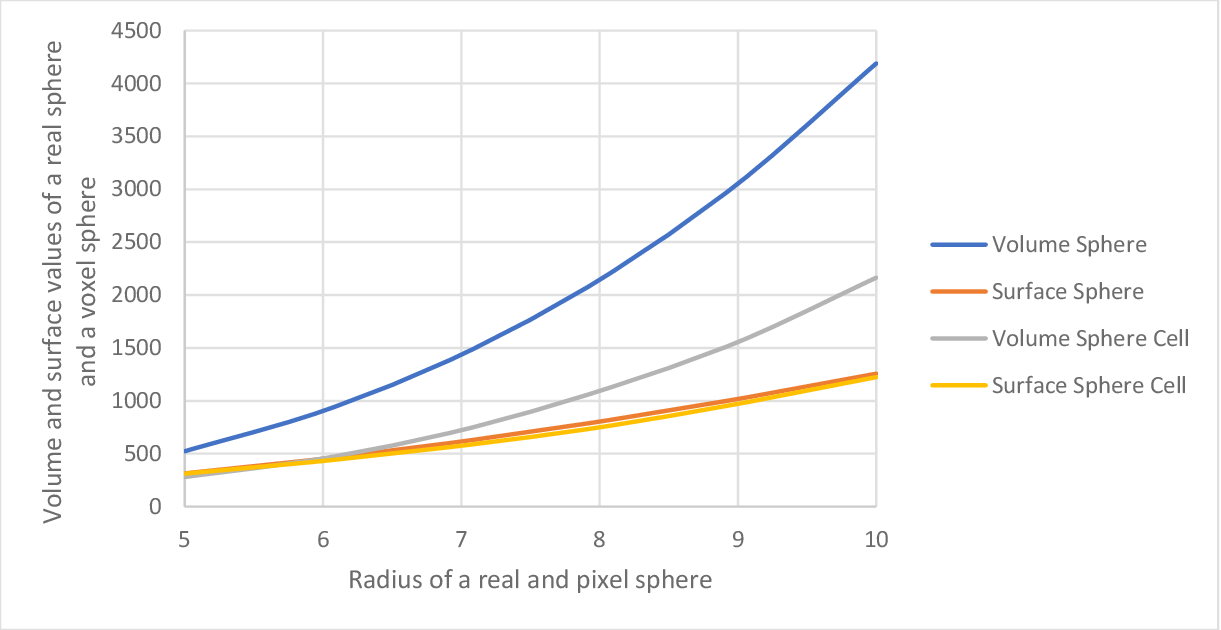
\includegraphics[scale=0.3]{figures/DeviationSphereToPixelSphere-vD0_8.png}
	\caption[Volume and surface in \SI{}{\micro\metre} between a sphere and a sphere cell for a voxel density of 0.8]{Volume and surface in \SI{}{\micro\metre} between a sphere and a sphere cell for a voxel density of 0.8.  The lines 'Volume Sphere' and 'Surface Sphere' are displaying the volume and the surface of a sphere. The lines 'Volume Sphere Cell' and 'Surface Sphere Cell' display the volume and the surface of a sphere cell.}
	\label{img:DeviationSphereCellRealSphere-vD0,8}
\end{figure}

\begin{figure}[ht]
	\center
	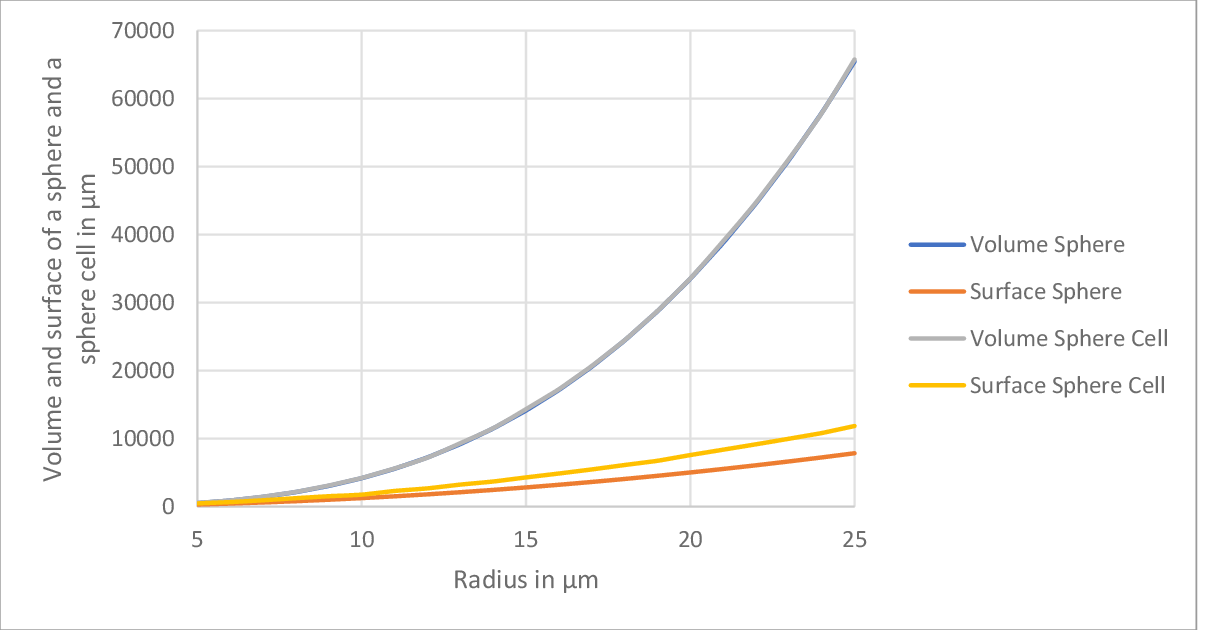
\includegraphics[scale=0.3]{figures/DeviationSphereToPixelSphere-vD1.png}
	\caption[Volume and surface in \SI{}{\micro\metre} between a sphere and a sphere cell for a voxel density of 1]{Volume and surface in \SI{}{\micro\metre} between a sphere and a sphere cell for a voxel density of 1.  The lines 'Volume Sphere' and 'Surface Sphere' are displaying the volume and the surface of a sphere. The lines 'Volume Sphere Cell' and 'Surface Sphere Cell' display the volume and the surface of a sphere cell. The line 'Volume Sphere' is not visible because it lays under the line 'Volume Sphere Cell'. The deviation between these values is so small that only one line is displayed.}
	\label{img:DeviationSphereCellRealSphere-vD1}
\end{figure}

\section{Surface approximation}
The approximation of the surface of a cell to a surface of a real sphere is done with voxels, because these are also used in the simulation field. There are other techniques to approximate the surface of a sphere. It is possible to use pyramids for this approximation. Since in the current simulation the square lattice is used it might is difficult to find an approximation technique which suits the square lattice better. Moreover, the volumes of the cells and of a sphere are almost identical for the same radius, if the voxel density is 1. Because the volume of a cell is more important than the correct surface ,as it is listed in table \ref{tbl:CellConstraints} at page \pageref{tbl:CellConstraints}, a new approximatino has to be checked against its volume as well as its surface. The use of pyramids might be in general a great way to approximate a sphere but for the square lattice it might be not as suited as it uses cuboids.

\section{Surface Variation Pixels to Sphere}
The created algorithm of section \ref{sec:CreatedAlgorithm} has its benefits and also its weaknesses. There are several ways to design the algorithm. One is to use the same method as it is used to draw the sphere cell. With this method every voxel in the cuboid has to be checked if it is inside or outside the algorithm. Therefore, a lot of calculations are required just to create matrix of the cuboid, with the radius two times larger than the one of the sphere, from which the volume and surface sites can be calculated. This amount of calculations is $r^{3}$, where the radius of the cuboid is $2 \cdot r$, as it is explained in section \ref{sec:DrawSphereCells}. Thus, the amount of calculations to create the algorithm is $(2 \cdot r)^{3}$, where $r$ is the radius of the sphere. Because this approach has a high computational cost it should be only used if it is necessary. \newline
The next two approaches are similiar. Both split the cuboid and the circle up into eight pieces, then the calculations are done with one of the eight cuboids and as last step this result gets mirrored. This is possible because a cuboid split up into an odd amount of parts creates several smaller cuboids. With this small cuboid it is possible to calculate if every cuboid, in the small cuboid, is inside the sphere. Then the matrix is created. For the calculation of the volume and surface the result of the one eigth of the cuboid is mirrored for all three axes. This approach has less computations than the approach before. The amount of computations is now $(\dfrac{r}{2})^{3}$. Because only the half of the radius of the sphere is used, this is an improvement over the approach before. \newline
The approach with the least computational cost is similiar to the one before. After the cuboid around the sphere is split up into eight pices, the point in which the circle is at a given x,z coordinate is calculated. Then it is checked which cuboids at this given x,z coordinate are within the circle or not. Based on this approach there are even less calculations. Because of the eigth of the cuboid only the height of the circle for a given x,z coordinate is calculated. The required amount of calculations is now $(\dfrac{r}{2})^{2}$. Because one eigth of the cuboid is used, the half of the radius of the sphere is required. Moreover, only every x,z coordinate is needed for the calculations, instead of every x,y,z coordinate of the cuboids. Thus, the approach of the algorithm has the lowest computational cost. Even the algorithm has its weakness, it has a good basis to be further developed.

\section{Simulation Results}\label{sec:SimulationResults}
During this bachelor thesis one simulation has been finished. This simulation took 14 days to complete, therefore no other simulation had a complete simulation run. Other simulations were simulated 20 up to 50 days. First the completed simulation will be discussed and then aspects of the other simulations are included. \newline
It is interesting to see that both fitness functions have an increase after almost one year, as it is displayed in figure \ref{img:Fa_Fv_SPA/BCPD/IPCD} at page \pageref{img:Fa_Fv_SPA/BCPD/IPCD}. Why this increase happens for both fitness functions at the same point is a puzzle. The problem is that only the cells at the edges and sites are visible but there is no quick overview of the inside of the simulate urothelium. Another interesting fact is that the simulated urothelium has in the middle less cells than at the edges of the urothelium. This might be a result of the urination event, as the cells which are removed are randomly choosen. It would be interesting to see if this happens for other simulations as well or if this happend by incident. \newline
A similiarity of all simulations is that the result of the arrangement fitness function always decreases in the first 50 days. Because in the finished simulation this is also the case and it increases later in the simulation it might be normal in the simulation. No statement can be done if this decrease of the arrangement fitness function is normal or not. For the result of the volume fitness function no similiarities of the different simulation runs were found. Maybe there would be some similiarites visible for a longer duration of the simulations.

\section{CC3D}
Several simulation programs have been tested in an earlier master thesis of the project \cite{MSCAngelo}, it was evidenced that \ac{CC3D} is the best suited program. During this bachelor thesis several weaknesses of \ac{CC3D} are realized which are explained in the following paragraph. \newline
To develop a program an debugger should be available. An debugger allows the developer to execute the program command wise and to observe the values of the variables in the program. \ac{CC3D} do not offer an debugger. Therefore every observation of a variable or the order of the function calls has to be printed to the command line. This has signifacant disadvantages, as it requires more time to understand the structure of the code as well as the print commands first have to be written. Moreover, the developer has to be very precise at the print commands and she / he needs to know which output at the command line belongs to which print command. \newline
A second disadvantage is that the memory after an simulation is not released. Every simulation requires an specific amount of memory dependent of the simulation field size. This memory should be released after the simulation is finished. If the memory would be released after the simulation other programs could use it. Moreover, by starting a simulation after another simulation is finished, \ac{CC3D} reserves the memory for the new simulation in addition to the required simulation before. Therefore, by starting several simulations without closing \ac{CC3D}, the program has a high probability to crash because there is not enough memory free for the simulation. \newline
Because the required memory for an simulation increases as the size of the simulation field increases it is good to know where the constraints of the size of the simulation field are. The size constraints was tested on an \ac{VM} with the distribution 'Windows 7' as an 64 bit version. The \ac{VM} has a memory of 4GB. For this memory the constraint of the size of the simulation field is around by 400 voxels for each axis. Therefore, around 107171875 voxels are allowed in the simulation. For this size of the simulation field \ac{CC3D} became very slow, which is a result of the amount of memory. This constraint is different for different distributions as well as for different sizes of the memory. 

\section{GGH Model}
The \ac{GGH} model is widely used because it is easy to use. Even it is easy to use some parameters of the approach are not explained in detailed. As example it is possible to set a temperature for the simulation. This temperature effects how much a cell fluctuates as it changes its volume or surface. That the fluctuations changes with a different temperature is observable. Because it is almost nowhere explained it is questionable if this is the only effect of the temperature in the simulation or are the other effects with it. \newline
For the scenario with the sphere cell it is a disadvantage that it is not possible to set a constraint of the shape of a cell. The use of one radius or one diameter would already be enough to limit the amount of possible shapes of a cell for a given volume and surface. Because such a constraint can not be set and it is not explained in the literature how to receive a specific shape of a cell a lot of experiments has to be done to reach the desired shape of the cell.